
\chapter{Intermediate Representation}
\label{ch-ir}

{\small
\begin{flushright}
Design: Cristina and Mike[c.96-98]; 
Documentation: Cristina [c.1998, May 00], Mike [May 00], Brian [Oct 01]
\end{flushright} 
}

The intermediate representation is a combination of various
data structures to manipulate machine instructions in an
abstract way, and to allow analyses to be performed on those
instructions. 

The intermediate representation used in \uqbt\ is composed of:
\begin{itemize}
\item Register transfer lists (\rtl s) that represent the assembly
instructions of the machine.  \rtl s are converted into a higher-level 
representation called \hrtl\ by means of transformations 
(explained in Part~\ref{part-analysis}).  
The \rtl\ language is described in Section~\ref{sec-rtl}, and
the \hrtl\ language is described in Section~\ref{sec-hrtl}.

\item Control flow graph of basic blocks for each procedure\footnote{
Throughout this document, the word {\it procedure} refers to a
subroutine; that is, a subroutine that returns a value (i.e. function) 
or a subroutine that does not return a value (i.e. procedure).
} in the program.
The construction of control flow graphs is described in Section~\ref{sec-cfg}.
\end{itemize}

The main data structures used to represent a program are illustrated
in Figure~\ref{fig-datastructs} and follow this hierarchy:
\begin{itemize}
\item A program is represented by a \prog\ structure which holds
general information about the input binary executable.
This information is setup by the loader while decoding the
binary-file (e.g. entry point, pointers to .text and .data segments,
dynamic information, etc).

A program is a collection of procedures; these procedures are
stored in a list.

\item A procedure is represented by a \proc\ structure which holds
general information about a procedure (e.g. entry point, size (in bytes)
of the procedure, name (if known), etc).

A procedure is represented by a control flow graph and its register
transfer list instructions.

\item A control flow graph (CFG) of basic blocks (BBs) is represented by
a \bb\ structure which holds information about the one basic
block (e.g. entry point, pointers to first and last instructions
in the BB, type of BB, successors (i.e. out-edges), predecessors (i.e.
in-edges), number of out-edges, number of in-edges, etc).

A BB has links to the first and last RTL instructions that belong to
the BB, rather than including the RTL instructions itself.

\item A register transfer language (RTL) instruction is represented
by an \rtl\ structure which holds precise information about the
machine instruction (e.g. type of instruction, condition codes set,
condition codes used, registers set, registers used, etc).
\end{itemize}

% xfig figure exported as eps, 100% size, portrait, displayed at 6cm height
\centerfigbegin
\resizebox{!}{6cm}
{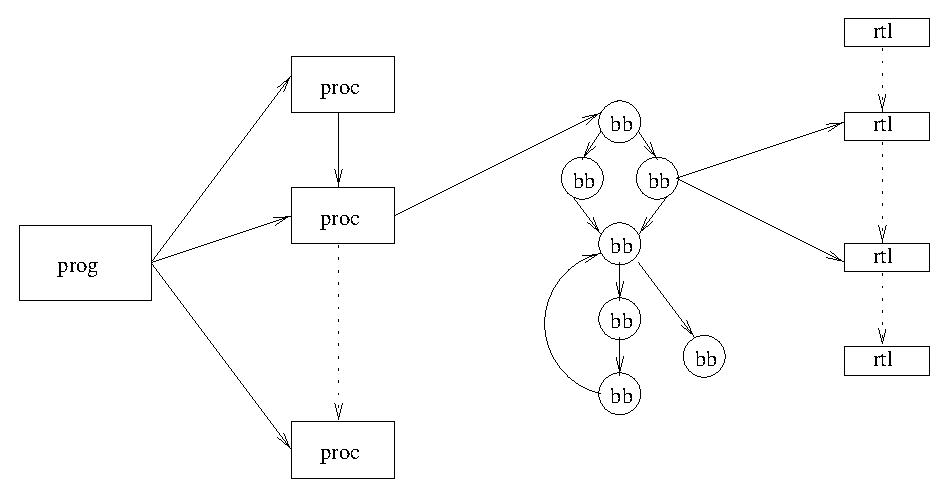
\includegraphics{figures/datastructs.eps}}
\centerfigend{fig-datastructs}{Data Structures to Represent a Binary Program}

We describe each of these parts of the intermediate representation
in reverse order, that is, starting from atomic data structures
and ending up with the program structure.



\section{Register Transfer Lists}
\label{sec-rtl}

{\small
\begin{flushright}
Design: Cristina, Mike; Documentation: Cristina, Doug, Mike;
 Implementation: Doug, David, Mike
\end{flushright} 
}

UQBT uses a simple, low-level register-transfer representation for the
effects of machine instructions.
A single instruction corresponds to a register-transfer list or RTL,
which in UQBT is a sequential composition of effects.
Each effect assigns an expression to a location.
All side effects are explicit at the top level;
expressions are evaluated without side effects, using purely
functional \emph{RTL operators}.
For example, the effects of the SPARC \texttt{call} instruction are
represented by the following RTL:

\begin{smallverbatim}
r[15] := %pc
%pc   := %npc
%npc  := r[15] + (4 * disp30)
\end{smallverbatim}
This sequence of effect puts the program counter~\texttt{\%pc} in
register~15, copies the ``next program counter''~\texttt{\%npc} into
the program counter, and puts the target address into~\texttt{\%npc}.
Because the target address is computed relative to the \emph{original}
program counter, the target-address computation uses register~15,
which holds the original value of~\texttt{\%pc}.
Because the SPARC uses delayed branches,  the target address
is placed into \texttt{\%npc}, not directly into \texttt{\%pc}.

Register transfer lists (RTLs) capture the semantic information 
of machine instructions by means of a series of \emph{effects} on a 
\emph{location}.
One register transfer is an assignment of an expression (i.e. an 
effect) to a location (i.e. a register or memory).  
There are no side effects, all effects are explicitly mentioned in 
the RTL.
The RTL environment assumes an infinite number of registers and
infinite memory space.  Memory is a sequence of bytes.  
{\it We will need specialized types of memory, such as memory for 
local variables, once the analysis has been formalized.   We
will do that then, so for now, there is only one type of memory. }

An `RTL language' is defined by a collection of locations and
operators.
UQBT uses an RTL language defined by taking the union of locations on
machines M$_S$ and M$_T$ and the union of the operators used in the
descriptions of machine M$_S$ and M$_T$.
The `machine~$X$ invariant' defines a sub-language of RTLs called
the $X$-RTLs; an RTL is an $X$-RTL if and only if it can be represented
as a single instruction on machine~$X$.

\uqbt 's \rtl\ implements the semantic information expressed in SSL
notation (SSL is described in Chapter~\ref{ch-ssl}).  

\subsection{Types}
\label{sec-rtltypes}
We define the following types to work with RTLs.  
(NOTE that these names should be in uppercase and perhaps shorter.
I've listed them as they appear in the rtl.h interface so that we don't
get confused -- when those are updated, these should be updated).
\begin{description}
\item[RTlist] a list of register transfers. Various analysis
    functions work on RTlists, such as GetControlTransfer().

\item[RTLInstDict] a dictionary of expanded instructions from the SSL
    file.

\item[RT] a register transfer is an assignment statement
    which has a variable (i.e. location) as the left-hand
    side and an expression (i.e. value) on the right-hand side. \\
    {\it We have considered introducing in the future a specialized
    RT which is a call, but at present that has not been decided
    upon.  We think it will be useful for analysis purposes. }

\item[RTAssgn] a subclass of class RT, representing an RT assignment
    (i.e. location := expression). One instruction may have zero
    (for NOP only) or more of these.

\item[RTFlagDef] a subclass of class RT, representing the definition
     of a flag function.

\item[RTFlagCall] a subclass of class RT, representing the call to a
    flag function.

\item[SemStr] a Semantic String, which is a prefix linearisation of an
    expression tree (see below).
    A SemStr can be used to represent a location, value, or subexpression.

    Expression operators are reproduced in Figure~\ref{fig-expOps2}.

% I'm not sure what this was meant to be about... probably some restriction
% on expressions which has long faded from the code. I keep it in comments
% in case it's not what I think it is. MVE
\begin{comment}
    {\it This may need to go elsewhere - Mike}
    An address expression is constrained to plus or minus offsets 
    from an address, hence the case \texttt{M[reg + reg * kte]} is not 
    supported directly; a subexpression needs to be computed into a 
    register and used as a register index in this case.

    These 3 options can be represented by 2: registers or constants.
    When an address expression is received, it is computed into 
    a register and that register is used to index into memory. 
    In this way we do not constrain address expressions (given that
    other machines may have more complicated addressing modes) 
    and create a simpler interface.
\end{comment}

\end{description}

\centerfigbegin
\begin{tabular}{|l|l|c|c|c|l|l|} \hline
Type of Operator & Id       &
\multicolumn{3}{c|}{Arguments}
& Symbol    & Meaning \\ \cline{3-5}
    &   & Int & Fix & Var & & \\
\hline
unary       & idNot         &0&0&1  & \verb!~!  & logical not \\
            & idNeg         &0&0&1  & 0-        & unary minus \\
\hline
binary      & idPlus        &0&0&2  & +         & addition \\
            & idMinus       &0&0&2  & -         & subtraction \\
            & idMult        &0&0&2  & *         & multiplication (unsigned)\\
            & idMults       &0&0&2  & *!        & multiplication (unsigned)\\
            & idDiv         &0&0&2  & /         & division (signed) \\
            & idDivs        &0&0&2  & /!        & division (signed) \\
            & idMod         &0&0&2  & \%        & modulus (unsigned) \\ 
            & idMods        &0&0&2  & \%!       & modulus (signed) \\ 
            & idBitAnd      &0&0&2  & \&        & (bitwise) and \\
%           & idBitAndNot   &0&0&2  & \&\~      & (bitwise) and-not \\
            & idBitOr       &0&0&2  & $|$       & (bitwise) or \\
%           & idOrNot       &0&0&2  & $|$\~     & (bitwise) or-not \\
            & idBitXor      &0&0&2  & \verb!^!  & xor \\
%           & idBitXorNot   &0&0&2  & \verb!^~! & xor-not \\
            & idShiftR      &0&0&2  & $>>$      & right-shift \\
            & idShiftL      &0&0&2  & $<<$      & left-shift \\
            & idShiftRA     &0&0&2  & $>>$A     & right-shift-arithmetic \\
            & idRotateL     &0&0&2  & rl        & rotate-left \\
            & idRotateR     &0&0&2  & rr        & rotate-right \\
            & idRotateLC    &0&0&2  & rlc       & rotate-left-through-carry \\
            & idRotateRC    &0&0&2  & rrc       & rotate-right-through-carry \\
\hline
ternary     & idTern        &0&0&3  & ?:        & c-style ternary \\
            & idAt          &0&0&3  & @         & bit extraction \\
\hline
logical     & idEquals      &0&0&2  & =         & equal \\
            & idNotEqual    &0&0&2  & \verb!~=! & not equal \\
            & idLess        &0&0&2  & $<$       & less than, signed \\
            & idGreater     &0&0&2  & $>$       & greater than, signed \\
            & idLessEq      &0&0&2  & $<=$      & less or equal to, signed \\
            & idGreaterEq   &0&0&2  & $>=$      & greater or equal to, signed \\
            & idLessUns     &0&0&2  & $<$u      & less than, unsigned \\
            & idGtrUns      &0&0&2  & $>$u      & greater than, unsigned \\
            & idLessEqUns   &0&0&2  & $<=$u     & less or equal to, unsigned \\
            & idGtrEqUns    &0&0&2  & $>=$u     & greater or equals, unsigned \\
            & idAnd         &0&0&2  & and       & and (of two expressions) \\
            & idOr          &0&0&2  & or        & or \\
\hline
operations  & idMemOf       &0&0&1  & m[...]    & memory of \\
            & idRegOf       &0&0&1  & r[...]    & register of \\
            & idAddrOf      &0&0&1  & a[...]    & address of (cancels m[]) \\
            & idVar         &1&0&0  & v\it{n}   & variable; replaces reg or mem \\
            & idParam       &0&1&0  & param`...'& parameter \\
            & idRparam      &0&1&0  & rparam`...'& register parameter \\
            & idExpand      &0&1&0  & expand`...'& expand (not for user) \\
            & idTemp        &0&1&0  & temp`...' & temporary register \\
            & idSize        &1&0&1  & size \it{n}& size cast \\
            & idDef         &0&1&0  & def `...' & definition; special for UQDBT \\
            & idIndex       &0&0&2  & [...]     & special for UQDBT \\
\hline
constants   & idIntConst    &1&0&0  & int \it{n}& integer constant \\
            & idFloatConst  &2&0&0  & float \it{f}& floating point constant \\
\hline
\end{tabular}
\centerfigend{fig-expOps2}{Expression Operators for RTL (cont over page)}

\centerfigbegin
\begin{tabular}{|l|l|c|c|c|l|l|} \hline
Type of Operator & Id       &
\multicolumn{3}{c|}{Arguments}
& Symbol    & Meaning \\ \cline{3-5}
    &   & Int & Fix & Var & & \\
\hline
type conversions& idSignExt &0&0&1  & !         & sign-extend (no sizes) \\
            & idTrunc       &2&0&1  & trunc(\it{exp, s1, s2})& truncate from s1 to s2 bits \\
            & idZfill       &2&0&1  & zfill(\it{exp, s1, s2})& zero fill from s1 to s2 bits \\
            & idSgnEx       &2&0&1  & sgnex(\it{exp, s1, s2})& sign extend from s1 to s2 bits \\
\hline
float conversions&idFsize   &2&0&1  & fsize(\it{exp, s1, s2})& float size convert from s1 to s2 \\
            & idItof        &2&0&1  & itof(\it{exp, s1, s2})& integer to float, s1 to s2 bits \\
            & idFtoi        &2&0&1  & ftoi(\it{exp, s1, s2})& float to integer, s1 to s2 bits \\
            & idFround      &2&0&1  & fround(\it{exp, s1, s2})& float round, s1 to s2 bits \\
\hline
\end{tabular}
\centerfigend{fig-expOps2a}{Expression Operators for RTL (cont from prev page)}

\subsection{Interface Functions to Create and Use RTLs}
All objects have constructor and destructor functions, as well
as functions to access elements of an object.  
Specialized analysis-related functions are explained in the
last subsection of this section---Functions for Analysis 
Purposes.  \\
{\it This style file doesn't number subsub sections,
how annoying! }


\subsubsection{Semantic String Class}
A semantic string object (SemStr) is a prefix linearisation of a tree
of RT components, such as constants, registers, memory, and various
expressions involving these. It is inplemented as a list of integers
(called items);
many of these integers are indices into a special table called the
Semantic Table. Entries in this table represent various things, such
as operators, special registers, parameters, and so on.

Here are a few examples: index 0 (the first entry) is called \texttt{idPlus},
and represents binary addition. Approximately index 75 is called
\texttt{idIntConst}, representing an integer (the actual integer is the next
integer in the string, following the {\tt idIntConst}).  So the expression
\texttt{2+2} is represented by the string ``{\tt 0 75 2 75 2}'' (read this
as ``plus int 2 int 2''). 

All the operators listed in Figure~\ref{fig-expOps2} are automatically
included in the table, and they are
machine independent. Special registers (e.g. the Next Program Counter register
({\tt \%npc}) and parameters (e.g. {\tt rs1} for the first source
register) are added
by the parser of the SSL file (see Chapter~\ref{ch-ssl}).
Let's consider a complete RTAssgn, conventionally written as

{\tt r[4] = m[1000] + 5}

This will be implemented as two semantic strings, one for the
location (left hand side) and one for the value (right hand side).
Each will be a list of integers, which might be

{\tt 34 75 4} ~~~and~~~ {\tt 0 38 75 1000 75 5}

and might print as

{\tt r[4]} ~~~and~~~   {\tt m[1000] + 5}  ~~~normally (the "int" is dropped
for brevity), or

{\tt r[ int 4]}  ~~~and~~~  {\tt + m[ int 1000 ] int 5}

if you choose to use the printPrefix() member function. This latter
representation is better for debugging problems with semantic strings,
though obviously it is less readable.

The first SemStr could be read as ``RegOf int 4''. The first integer, 34,
is an index into the semantic table, where among other information
there is the string ``r['' (for the SemStr print routine).
The enumerated constant ``idRegOf'' can be used in programs to
represent this index (see Figure~\ref{fig-expOps2} for a complete list
of these enumerated constants). The second integer,
75, is also an index into the semantic table, and says that the integer
following this index is to be taken as a literal integer. The third
integer, 4, represents itself. The second semantic string is a little
more complex. Its first index, 0, represents addition. The two arguments
to be added come next, but they are variable length. Immediately after
the 0 is 38, representing "memory of". The thing following the MemOf
could be any kind of expression; in this case it's ``int 1000'', but
it could have been say ``{\tt+ 500 500}'', or ``{\tt - r[ int 16 int 8}''.

Note that special registers (such as {\tt \%pc} or {\tt \%CF}) are
represented differently from general purpose registers. General purpose
registers are numbered, whereas special registers have their own
index into the semantic table (see Section~\ref{sec-semtable}).

A word on nomenclature: the word {\it parameter} is used to describe
a part of an instruction that will be {\it instantiated} with the
RTL function. For example, ``regorimm'' could be a parameter representing
a part of an instruction; actual values could be ``r[4]'' or ``4''.
The word {\it argument} is used here to mean those parts of a semantic
string that represent arguments (or operands) to the first index. For example,
if the first index is {\tt idMinus}, then there are two variable length
arguments to it, representing the minuend and the subtrahend respectively.
If the first index is idSize, there is one integer argument (the number
of bits in the size being cast to), and one variable length argument
(the expression being size cast).

Every semantic string has a type (e.g. unsigned integer 32 bits); the type is
represented by class Type (see Section~\ref{sec-class-type}). If not explicitly
specified, the semantic string is assigned the default type (which is signed
integer 32 bits). This type is preserved when semantic strings are copied,
subexpressions are made, and so on.

\begin{itemize}
\item   SemStr: $\emptyset$ \ra SemStr.
    Default constructor.

\item   SemStr: Kind \ra SemStr.
    Constructor that takes an expression kind. The kinds are only these:
    uORDINARY, eOPTABLE, and eCONDTABLE. Not for users.

\item   SemStr: SemStr \ra SemStr.
    Copy constructor.

\item   operator=: SemStr \ra SemStr.
    Assignment operator.

\item   SemStr: (Iterator1 x Iterator2) \ra SemStr.
    Constructor that takes a pair of iterators. Makes a copy of part
    of some other SemStr starting with the item referenced by iterator1
    up to but not including iterator2.

\item   SemStr: (int* x int* x Kind) \ra SemStr.
    Constructor that takes two pointers to an array of integers (pointer to
    first and pointer to last). Also takes kind, as above.

\item   getKind: SemStr \ra Kind.
    Gets the kind as above. Not for users.

\item   getType: SemStr \ra Type.
    Gets the type (as class Type) for the semantic string.

\item   isFloat: SemStr \ra BOOL.
    Note: deprecated. Returns true if the expression this semantic string
    represents is a floating point type.

\item   setType: (SemStr x Type) \ra $\emptyset$.
    Set the type for the expression that this semantic string represents.

\item   setTypes: (SemStr x SemStr) \ra $\emptyset$.
    Set the type for this semantic string to be the same as the type of the
    given semantic string.

\item   operator==: (SemStr x SemStr) \ra BOOL.
    Returns true if this SemStr is equal to the given SemStr. Type is taken
    into account in the comparison.

\item   operator\%=: (SemStr x SemStr) \ra BOOL.
    Same as above, except that type is \emph{not} taken into account.

\item   operator-=: (SemStr x SemStr) \ra BOOL.
    Same as the two above, except that only the sign element of the type is
    disregarded. Therefore, to return true, the expressions must match, and
    the size and broad type must match, but the ``signedness'' need not
    match.

\item   operator$<$: (SemStr x SemStr) \ra BOOL.
    Returns true if this SemStr is ``less than'' the given SemStr. Comparison
    is arbitrary, but establises a unique ordering of semantic strings. This
    function is often used implictly where there are maps of semantic strings.
    Type is included in the comparison.

\item   operator$<<$: (SemStr x SemStr) \ra BOOL
    Same as the above, except that ``signedness'' is not considered in the
    comparison.

\item   push: (SemStr x int) \ra $\emptyset$.
    Push the given integer to the end of the semantic string. It is up to
    the user to make sure that the semantic string is valid.

\item   prep: (SemStr x int) \ra $\emptyset$.
    Prepend the given integer to the front of the semantic string. It is
    up to the user to make sure that the semantic string is valid.

\item   pushSS: (SemStr x SemStr) \ra $\emptyset$.
    Push a copy of the given semantic string to the end of this string

\item   pushArr: (SemStr x int x int*) \ra $\emptyset$.
    Push the given number of integers from the given array of integers to
    the end of the string.

\item   pop: $\emptyset$ \ra int.
    Remove the last integer from the list, and return it.

\item   popFirst: $\emptyset$ \ra int.
    Remove the first integer from the list, and return it.

\item   clear: $\emptyset$ \ra $\emptyset$.
    Set this semantic string to be empty (no elements in the list).

\item   isSpRegEqual: (SemStr x int) \ra BOOL.
    Returns true if this semantic string matches the special register
    whose index is given. Not for most users.

\item   isSpRegCont: (SemStr x int) \ra BOOL.
    Returns true if this semantic string contains the special register
    whose index is given. Not for most users.

\item   isNumRegEqual: (SemStr x int) \ra BOOL.
    Returns true if this semantic string matches the register
    whose number is given. Not for most users.

\item   isNumRegCont: (SemStr x int) \ra BOOL.
    Returns true if this semantic string contains the register
    whose number is given. Not for most users.

\item   isArrayEqual: (SemStr x Array of int) \ra BOOL.
    Returns true if the elements of this semantic string match the
    elements of the given array of integers. Can be used to test for
    specific semantic strings, e.g. ``\%pc = \%npc''.

\item   getFirstIdx: SemStr \ra int.
    Returns the first item of this semantic string. Note that this really
    should be called getFirstItem, since the integer returned may not actually
    be an index (it could be an integer constant, or even half of a floating
    point constant).

\item   getSecondIdx: SemStr \ra int.
    Returns the second item of this semantic string. Usually used where
    the first index is known to contain one integer or fixed argument
    (e.g. the first index is idIntConst or idSize).

\item   getThirdIdx: SemStr \ra int.
    Returns the third item of this semantic string.

\item   getSubExpr: (SemStr x int) \ra SemStr*.
    Returns a pointer to a new semantic string, which is composed of
    the given subexpression. Passing zero returns the first argument
    to this expression, one returns the second, and so on.
    {\bf Note:} This member function only works with variable arguments.
    Use GetSecondIdx to access an integer or fixed argument.

\item   getSubExpr: (SemStr x int x SemStr) \ra SemStr.
    As above, but also stores the result in the reference (last) parameter.
    This ensures that the caller will automatically delete the semantic string
    when it goes out of scope.

\item   getIndex: (SemStr x int) \ra int.
    Get the {\it i}th item (where {\it i} is given).

\item   getLastIndex: SemStr \ra int.
    Get the last item of the list of integers in this semantic string.

    The next group of member functions concern searching for a subexpression
    withing this semantic string. An item of -1 in a semantic string is treated
    as a ``wildcard''.
    Formally, a search expression (S) will match a subexpression (E) if:

    length(S) $<=$ length(E) and for each position, p, in S the following holds:

    S[p] == -1 $||$ S[p] == E[p]

    Example: if {\it this} is \{0,\{3,78\},\{43,6,14\}\},
    it can be searched with the following subexpressions, and will return true:

\begin{tabular}{|l|l|} \hline
    Search & Result \\
\hline
    \{\{3,78\}\} & \{\{3,78\}\} \\
    \{\{0,*,*,\{43\}\}\} & \tt\{\{0,\{3,78\},\{43,6,14\}\}\} \\
\hline
\end{tabular}

\item   search: (SemStr x SemStr x SemStr x BOOL) \ra BOOL.
    Searches this semantic string for the given subexpression (first parameter
    after {\it this}). If found, the matching string is copied to the reference
    (last SemStr) parameter. The return value is whether a match was found.
    If the optional boolean is set, the search is type
    sensitive (i.e. the types have to match, as well as the expressions). This
    boolean defaults to false (i.e. the search defaults to case insensitive).

\item   searchAll: (SemStr x SemStr x list\{SemStr*\} x BOOL) \ra BOOL.
    Searches this semantic string for {\it all} occurrences of the given
    subexpression (first parameter after {\it this}). For each match, the
    matching string is appended to the list of pointers to semantic strings.
    The return value is whether any match was found.
    If the optional boolean is set, the search is type
    sensitive (i.e. the types have to match, as well as the expressions). This
    boolean defaults to false (i.e. the search defaults to case insensitive).

\item   searchReplace: (SemStr x SemStr x SemStr x BOOL) \ra BOOL.
    Searches this semantic string for the given subexpression (first parameter
    after {\it this}). If found, the matching string is replaced by the
    reference (last SemStr) parameter. The return value is whether a match was
    found.
    If the optional boolean is set, the search is type
    sensitive (i.e. the types have to match, as well as the expressions). This
    boolean defaults to false (i.e. the search defaults to case insensitive).

\item   searchReplaceAll: (SemStr x SemStr x SemStr x BOOL) \ra BOOL.
    Searches this semantic string for {\it all} occurrences of the given
    subexpression (first parameter after {\it this}). For each match, the
    matching string is replaced by the given string (last SemStr parameter).
    The return value is whether any replacement was made.
    If the optional boolean is set, the search is type
    sensitive (i.e. the types have to match, as well as the expressions). This
    boolean defaults to false (i.e. the search defaults to case insensitive).

\item   substReg: (SemStr x int x SemStr) \ra BOOL.
    Substitute all occurrences of the given numbered register with the given
    semantic string. Returns true if any match found.
 
\item   substSpcl: (SemStr x int x SemStr) \ra BOOL.
    Substitute all occurrences of the given special register (index is given)
    with the given semantic string.

\item   substIndex: (SemStr x int x int) \ra $\emptyset$
    Replace the item at the given index with the given integer. For example,
    substIndex(0, 77) will replace the first item in the list with 77.
 
\item   smartCompare: (SemStr x SemStr x BOOL x list\{int\}) \ra BOOL.
    This function is not complete. Do not use.

\item   findEndSubExpr(SemStr x iterator) \ra iterator.
    Given an iterator into this semantic string, step forward towards the end
    of this string until the end of the subexpression headed by the given
    iterator is found. Returns an iterator that is just past the end of that
    subexpression. For example, if given (3+4)*(5+6) (internally
    * + int 3 int 4 + int 5 int 6), with an iterator pointing to the first
    plus, returns an iterator to the second plus (just past the (3+4)
    subexpression).
    There are actually two functions with the same name; one takes and
    returns a const iterator, and one takes and returns a non-const iterator.

\item   simplify: SemStr \ra $\emptyset$
    Simplify this expression using constant folding and the like, and also
    cannonicalising the expression by placing integer constants on the
    right if possible (so 2+a is replaced by a+2). a + -2 is replaced by a-2.
    a $<<$ k is changed to a * K where K=2**k.

\item   findSubExpr: (SemStr x int x int* x int) \ra BOOL.
    Search this semantic string for the expression (given by the given number
    of integers in the given array of integers). Returns true if found. If
    found and there were wildcards in the array, the item matched by the last
    wildcard is written to the reference (last) parameter.

\item   sprint: SemStr \ra string.
    Prints a representation of this semantic string to a string, which
    is returned. This is a conventional (infix) representation, and
    so it somewhat removed from the actual (prefix) implementation.
    Some effort is made to pretty the result, e.g. r[ int 4] is
    displayed as r[4].
    When exact knowledge of the format of the string is required, use
    sprintPrefix below.

\item   print: (SemStr x ostream) \ra $\emptyset$.
    Prints a representation of the semantic string to the given stream,
    or to cout if none is given. It is equivalent to printing the string
    returned by sprint to the given stream.

\item   sprintPrefix: SemStr \ra string.
    Prints a representation of this semantic string to a string, which
    is returned. The format is strongly tied to the internal (prefix)
    representation of the semantic string, so it is harder to read than
    the result from sprint, but may be more useful for debugging.

\item   printPrefix: (SemStr x ostream) \ra $\emptyset$.
    Prints a representation of the semantic string to the given stream,
    or to cout if none is given. It is equivalent to printing the string
    returned by sprintPrefix to the given stream.

\item   len: SemStr \ra int.
    Returns the number of items in this semantic string.

\item   instantiate: (SemStr x list\{int\} x vector\{char*\} x RMAP) \ra BOOL.
    Replace all occurrences of formal instruction parameters (e.g. rs1) with
    actual expressions (e.g. r[12]). The last parameter is an object
    representing the register map. Not for users.

\end {itemize}

\subsubsection{Semantic Table Class}
\label{sec-semtable}

Semantic Strings (class SemStr) are mainly indices into a special
object of class SemTable, the semantic table. This is a global
object, accessable as {\tt theSemTable} as long as you
{\tt \#include "ss.h"}. Most of the time, the user need not be
concerned with the semantic table, but there are a few important
exceptions.

One of these is when dealing with special registers. These registers
are not accessed like general purpose registers (so called {\it numbered}
registers), but have their own entries in the semantic table. When
special registers are referenced in the SSL file (see Chapter~\ref{ch-ssl}),
they are placed into
the semantic table by the parser. The index of a particular special
register is not fixed (most of them are machine specific), so there is no
enumerated constant like {\tt idPlus} that can be used for a special
register. At present, the way to find an appropriate index is to use
the FindRegIndex member function.

\begin{itemize}
\item   findRegIndex: (SemTable x string) \ra int.
    Given the semantic table and a string representing the name of the
    special register (including the {\tt \%}), returns an integer index
    for the appropriate semantic table item. This single index
    represents the special register in semantic strings (compared with
    three integers for a numbered register).

\item   findOpIndex: (SemTable x char*) \ra int.
    Given a C string representing the operator (e.g. {\tt \verb!"&~"!}),
    returns the index representing the operator. This operator can be
    used to build expressions, etc. Note that this function is not
    efficient (at present, it uses a linear search), so it should not
    be used where the operator is known (in this case, {\tt idBitAndNot});
    use it where the operator could be one of a number of values, and
    only the string representation is known. (For example, the SSL
    parser uses this function when parsing SSL expressions).

\end{itemize}

\subsubsection{Type Class}
\label{sec-class-type}
Types inside Semantic Strings and elsewhere are represented by class Type.
A Type has three components: the broad type, sign, and size. The broad type
is given in terms of this enumerated type:

\begin{verbatim}
enum LOC_TYPE {
    VOID = 0,               // void (for return type only)
    INTEGER,                // integer (any size and signedness)
    FLOAT,                  // a floating point (any size)
    DATA_ADDRESS,           // a pointer to some data (e.g. char*, struct*,
                            // float* etc)
    FUNC_ADDRESS,           // a pointer to a function
    VARARGS,                // variable arguments from here on, i.e. "..."
    UNKNOWN
};
\end{verbatim}

A particular type is given by either a tuple (e.g. (INTEGER, unsigned, 32 bits))
or a couple (e.g. (FLOAT, 64 bits); the sign is irrelevant for a float, but
defaults to signed).

\begin{itemize}
\item   Type: $\emptyset$ \ra Type.
    Default constructor. Returns the default type, which is 32 bit signed
    integer.

\item   Type: (LOC\_TYPE x int x BOOL) \ra Type.
    Constructor, with type given as a LOC\_TYPE (see abvove), size in bits,
    and if the LOC\_TYPE is integer, a BOOL for sign (TRUE = signed).

\item   operator==: (Type x Type) \ra BOOL.
    Equality operator. Sign is considered in the comparison, so the types must
    match in all respects for this function to return TRUE.

\item   operator-=: (Type x Type) \ra BOOL.
    Equality operator. Sign is {\it not} considered, so for this function to
    return true, the broad types and size must match, but the sign need not.

\item   operator$<$: (Type x Type) \ra BOOL.
    Less than operator. Sign is considered in the comparison.
    This function establishes an arbitrary ordering among all types.

\item   operator$<<$: (Type x Type) \ra BOOL.
    Less than operator. Sign is {\it not} considered in the comparison.
    This function establishes an arbitrary ordering among all types.

\item   getSize: Type \ra int.
    Returns the size (in bits) component of the Type.

\item   getType: Type \ra LOC\_TYPE.
    Returns the Type component of the Type, as a LOC\_TYPE.

\item   getSize: Type \ra BOOL.
    Returns the sign component of the Type; TRUE if signed.

\item   setSize: (Type x int) \ra $\emptyset$.
    Sets the size (in bits) component of this Type.

\item   setType: (Type x LOC\_TYPE) \ra $\emptyset$.
    Sets the Type component of this Type, given a LOC\_TYPE.

\item   setSize: (Type x BOOL) \ra $\emptyset$.
    Sets the sign component of this Type; TRUE if signed.

\item   getCtype: Type \ra CHAR*.
    Returns a C-style null terminated string representing the C language
    equivalent of the type. For example, if the type is (integer, unsigned, 16)
    the returned string would be ``unsigned short''.

\end{itemize}


\subsubsection{Register Transfer Assignment Class}
A register transfer assignment (RTAssgn) object is an assignment of an
expression
to a location.  A register transfer object also has size information
to determine the number of bits of information transferred from
the expression to the location.

\begin{itemize}
\item  updateLHS: (RTAssgn x Location) \ra RT.
    Given an RT object and a location, the location
    information gets updated in the object.

\item  updateRHS: (RTAssgn x Expr) \ra RT.
    Given an RT object and an expression, the expression
    information gets updated in the object.

\item  updateSize: (RTAssgn x BYTE) \ra RT.
    Given an RT object and a size in bits, the size of the
    transfer information gets updated in the object.

\item  getLHS: RTAssgn \ra SemStr*.
    Given an RTAssgn object, returns a pointer to the semantic string
    representing the location of the assignment.

\item  getRHS: RTAssgn \ra SemStr*.
    Given an RTAssgn object, returns a pointer to the semantic string
    representing the expression of the assignment.

\item  getSize: RTAssgn \ra BYTE.
    Given an RT object, returns the size in bits of the transfer
    of information.
\end{itemize}


\subsubsection{Register Transfer List Object}
A register transfer list (RTlist) is a list of register transfer 
objects.  However, greater functionality is provided for this 
object for analysis purposes; those functions are described in the 
next section.
For traversal purposes, an RTlist keeps track of the `current'
register transfer being traversed (by default, the first one
in the list).

\begin{itemize}
\item RTlist: $\emptyset$ \ra RTlist.
    Constructor function which returns an empty object of type RTlist.

\item RTlist: (RTlist x RTlist) \ra RTlist.
    Copy constructor: given a source and destination RTlist 
    objects, copies the first one onto the second one.

\item insertRT: (RTlist x RT) \ra RTlist.
    Given an RTlist object and a register transfer, inserts the
    register transfer at the end of the list.

\item updateRT: (RTlist x RT x int) \ra RTlist.
    Given an RTlist object, a register transfer and an index position into
    a list, updates the indexed register transfer in the list
    with the new one (if possible), otherwise it does not modify
    the RTlist object.
\end{itemize}


\subsubsection{Functions for Analysis Purposes}
The following functions are required for analysis purposes and
are described per relevant object.
More functions will be added as we see fit.


\paragraph{Register Transfer Assignment Class}
Functions that allow users to know which registers are defined
and used in the register transfer.  Note that this information
is implicitly stored in the LHS and RHS fields of an 
RTAssgn object.

\begin{itemize}
\item  isSpRegDefined: (RTAssgn x int) \ra BOOL.
    Given a register transfer assignment object and an index representing
    a special register, returns 
    whether the register is defined in the assignment or not.

\item  isNumRegDefined: (RTAssgn x int) \ra BOOL.
    Given a register transfer assignment object and the number of a
    numbered register, returns whether that register was defined
    in the register transfer or not.

\item  isSpRegUsed: (RTAssgn x int) \ra BOOL.
    Given a register transfer assignment object and an index representing
    a special register, returns whether
    that register was used by the object or not.

\item  isNumRegUsed: (RTAssgn x int) \ra BOOL.
    Similar to IsRegUsed() but for a numbered register.

\item  numRegUse: RTAssgn \ra int.
    Given a register transfer object, returns the number of registers
    used by that transfer. \\
    {\it Not implemented at present. A similar function that returns a list of registers used may
    be useful. }

\item  numRegDef: RTAssgn \ra int.
    Given a register transfer object, returns the number of registers
    that were defined by that transfer. \\
    {\it Not implemented at present. A similar function that returns a list of registers defined may
    be useful. }
\end{itemize}


\paragraph{Register Transfer List Object} 
The RTlist object \emph{will} provide in the \emph{future} 
functions that allow us to quickly decide what type of 
instructions we are dealing with.  The following are two
such functions which are not currently implemented:

\begin{itemize}
\item RTL: (STRING x ADDRESS x ...) \ra RTlist.
    This function returns an instance of a register transfer
    list for a particular machine instruction.  The name
    of the instruction is a named used in the SSL specification,
    these names are normally the same names used in SLED
    specifications.   The given native address is the program counter's
    address and is stored for usage when building a control
    flow graph of the procedure (see Section~\ref{sec-cfg}). \\ 
    The function returns an instance of an RTlist by reading
    the template file generated by SRD (refer to Section~\ref{sec-srd},
    Chapter~\ref{ch-ssl}).  \\

\item getBBSuccAddr: (RTlist x int) \ra ADDRESS.
    Given an RTlist object and an index position, returns the 
    address associated with that out-edge (if any) or Nil 
    otherwise.  \\
    This function is useful to construct a control flow graph,
    see example in Section~\ref{sec-cfg-eg}. 

\item getBBProcAddr: RTlist \ra ADDRESS.
    Given a call register transfer list, returns the target procedure 
    call address (if any) or Nil otherwise. \\
    This function is useful to construct a control flow graph,
    see example in Section~\ref{sec-cfg-eg}.

\item getNumRT: RTlist \ra int.
    Given an RTlist, returns the number of elements (RTs) in
    the list.

\item getRT: (RTlist x int) \ra RT.
    Given an RTlist object and an index into the list, returns
    the corresponding register transfer (if it exists) or 
    Nil.
    Elements in a list are indexed from one.

\item nextRT: RTlist \ra RT.
    Given an RTlist object, returns the next RT in the list (if any)
    or Nil (if at the end of the list).  The `current' index is
    updated to point to the next element in the list. 

\item isControlTransfer: RTlist \ra CTTYPE.
    Given an RTlist object, checks if the set of register 
    transfers are equivalent to a control transfer instruction,
    if so, returns the type of control transfer instruction 
    (one of ONEWAY, TWOWAY, NWAY, CALL, or FALL), otherwise
    returns NONE.  
    A control transfer instruction is one that explicitly 
    modifies the value of the program counter register.
\end{itemize}



\subsection{Usage of this Interface}
\label{sec-usageRTL}
A user can integrate RTL into a NJMC matching statement in
the following way: once an instruction has been decoded 
by matching one of the arms of the \texttt{match} statement, 
an instance of the matched instruction can be obtained in 
RTL form by passing the (unique) name of the instruction to
the RTL dictionary, along with the values of the other parts
of the instruction.  The RTL system will return an instance
of an entry in the dictionary. 
At present, the RTL instance function expects to receive 
the native address of the instruction being decoded, its name 
(i.e. key), and its arguments in string form.  The native 
address is required later on, for the purposes of constructing
a control flow graph of the program (see Section~\ref{sec-cfg}).

The following sample code illustrates the usage of this interface
with a SPARC matching statement.
The function \texttt{decode\_instr} implements a matching statement
which decodes the machine instruction pointed to by the \texttt{pc}
variable.  If the \texttt{alu} arm is matched, the \texttt{name} 
variable will hold the name of the arithmetic-logical instruction
matched.  The \texttt{RTLDisc.RTL} function is called with the
string values for the other parts of the arithmetic-logical 
instruction: the first register operand (\texttt{rs1}), the 
second register or immediate operand (matched in the \texttt{dis\_roi}
function), and the destination register \texttt{rd}).  Macros
are used (\texttt{RS1}, \texttt{ROI} and \texttt{RD}) to make
the translation from integer to strings depending on the context.
In the case of branch and call instructions, the target address passed
to the RTL dictionary is the \emph{raw} offset address given in the
instruction, rather than the relocated one; hence the need for the
equation provided to restore this value.  Alternatively, the 
core SLED spec for SPARC could be modified so that it does not 
relocate addresses automatically---this has not been done at 
present for consistency with disassemblers.

{\small
\begin{verbatim}
#define RD   (rd_names[rd])
#define RS1  (rs1_names[rs1])
#define RS2  (rs2_names[rs2])
#define ROI  (dis_roi(roi))

char *dis_roi(ADDRESS lc) {
  static char buf[512];
  match lc to
  | imode(i)   => sprintf(buf, "%d", i); return buf;
  | rmode(rs2) => return RS2;
  endmatch
}

void decode_instr (ADDRESS pc, ADDRESS uNativeAddr, RTLInstDict RTLDict, RTlist &rtl)
{
    match pc to
    | ...
    | alu (rs1, roi, rd) [name] => 
            rtl = RTLDict.RTL (uNativeAddr, name, RS1, ROI, RD);
    | branch^a (tgt, a) [name] => 
            sprintf(anulled, "%d", a);      // 1 if anulled
            rtl = RTLDict.RTL (uNativeAddr, name, numToStr((tgt-pc)>>2), anulled);
    | call_ (tgt) [name] => 
            rtl = RTLDict.RTL (uNativeAddr, name, numToStr((tgt-pc)>>2)); 
    | ...
    endmatch
\end{verbatim}  
}

This type of code (the whole matching statement file) can
obviously be mostly generated automatically, but at this stage we
either generate a decoder usingthe NJMC toolkit and modify that
code, or write it manually.


\section{Control Flow Graphs}
\label{sec-cfg}

{\small
\begin{flushright}
Design: Cristina; Documentation: Cristina; Implementation: Mike, Cristina
\end{flushright} 
}

A control flow graph (CFG) is a directed graph that represents the flow of 
control of a program, thus, it only represents the flow of instructions 
(code) of the program and excludes data information.
The nodes of a CFG represent basic blocks of the program, and the edges 
represent the flow of control between nodes.  More formally,

\begin{definition} \cite{Aho86}
\label{def-bb}
A {\bf basic block} is a sequence of consecutive statements in which
flow of control enters at the beginning and leaves at the end without
halt or possibility of branching except at the end.   
\end{definition}


\begin{definition}
\label{def-cfg}
A {\bf control flow graph} $G = (N,E,h)$ for a program $P$ is a connected,
directed graph, that satisfies the following conditions:
\begin{itemize}
\item $h$ is the unique entry node to the graph, 
\item $\forall \, n \in N, n$ represents a basic blocks of $P$, and 
\item $\forall \, e = (n_{i},n_{j}) \in E, e$ represents flow of control from
basic block $n_{i}$ to basic block $n_{j}$, and $n_{i}, n_{j} \in N$.
\end{itemize}
\end{definition}


\subsection{Types of Basic Blocks}
For the purposes of CFG construction, basic blocks are
classified into different types, according to the {\em last} instruction in 
the basic block.  Given that the instructions in the basic block
represent a sequential list of instructions (that would be executed
in that order), machine dependencies on the flow of control such as 
SPARC's delayed instructions cannot appear in the graph; they need
to be abstracted away into a machine-independent form.

Ideally, only 6 types of basic blocks are available.  However, 
during static decoding of a binary executable, it is not always
possible to determine the target branches of indirect and indexed
transfers of control.  In these cases, we make use of a node called
{\em nowhere} as the node does not lead to anywhere.  This node
will be analysed at runtime.  
The basic block types are: 

\begin{description}
\item [one-way] the last instruction in the basic block is an
unconditional jump to a known target location, hence, the block has one 
out-edge.

\item [two-way] the last instruction is a conditional jump to a 
known target location, thus, the block has two out-edges.

\item [n-way] the last instruction is an indexed/indirect jump to
known target locations.  The $n$ branches located in the index table become 
the $n$ out-edges of this node.

\item [call] the last instruction is a call to a procedure.
There are two out-edges from this block: one to the instruction following
the procedure call, and the other to the procedure that is called.
Throughout analyses, the called procedure is normally not followed,
unless interprocedural analysis is required.

\item [return] the last instruction is a procedure return instruction.
There are no out-edges from this basic block.

\item [fall] the next instruction is the target address of a
branch instruction (i.e. the next instruction has a label).  This node
is seen as a node that {\it falls through} the next one, thus, there is
only one out-edge.

\item [nowhere] the last instruction is an indexed or indirect jump
or call to an unknown target location.  This node has no out-edges. 
\end{description}


\subsection{Abstractions}
Based on definitions~\ref{def-bb} and \ref{def-cfg}, we define two 
abstractions to work with control flow graphs.

\begin{description}
\item [BB] is a basic block.  A BB holds information about the
    RTL instructions that form part of that basic block, as 
    well as successors of the basic block.

\item [CFG] is a control flow graph.  A CFG is a reference to 
    the header of the graph, i.e. a BB, and stores extra information
    like the state of the graph (see next section).
    Extra functionality is provided for a CFG which is not 
    provided for a BB, as seen in Section~\ref{sec-ir-cfg}.
\end{description}


\subsection{Steps in Constructing a CFG}
Machine instructions that modify the flow of control of a program 
have two types of references to the target address: via a machine-dependent
(physical) address, or via an offset into the stream of machine
instructions for the program.  Offsets resolve to physical 
addresses too.   
There are three main steps in the construction of the CFG:
\begin{enumerate}
\item Create a machine-dependent CFG by building BBs of instructions
    that contain native addressess for transfers of control.
\item Transform the machine-dependent CFG into a machine-independent
    CFG by transforming address references into edges (references
    to basic blocks).
\item Optimize the machine-independent CFG to remove extraneous 
    basic blocks introduced by limitations in the machine 
    instruction set (e.g. a jump to a jump), hence reducing the 
    number of nodes and edges of the graph. 
\end{enumerate} 

We will refer to the machine-independent CFG as a {\em well-formed} CFG
or \wfCFG.  This graph is the one used for analysis purposes. 


\subsection{Interface Functions to Construct Basic Blocks}
\label{sec-ir-bb}
Basic blocks have limited functionality: they can be 
constructed, and machine-dependent (i.e. host address) out-edges 
can be added to them. 

\begin{itemize}
\item BasicBlock: $\emptyset$ \ra BB.
    Constructor for a basic block.

\item addOutEdge: (BB x ADDRESS) \ra BOOL.  
    Adds the address as an out-edge in the given basic block. 
    The mapping between addresses and basic blocks is done when 
    the graph is well-formed.
    Returns true if successful.

\item addInterProcOutEdge (BB x ADDRESS) \ra BOOL.
    Adds an interprocedural out-edge to the basic block pBB that
    represents this address.  The mapping between addresses and
    basic blocks is done when the graph is well-formed.
    Returns true if successful.

\item addProcOutEdge: (BB x ADDRESS) \ra BOOL.
    Given a CALL basic block and an address of a procedure (i.e. the
    target address of a call instruction), stores the information
    in the basic block. 
    \emph{This function is not yet implemented.}
\end{itemize}


\subsection{Interface Functions to Construct a CFG}
\label{sec-ir-cfg}
Control flow graphs are composed of machine-dependent basic block nodes 
initially, and can then be transformed to machine-independent nodes
which are used for analysis purposes.  This latter graph is referred
to as a well-formed graph. 
A doubly-linked graph (i.e one that has in- and out-edges) can only be 
built once the graph is well-formed.
Further, a well-formed graph can be optimized to remove redundant edges 
and nodes (e.g. jumps to jumps).
The following functionality is provided by the interface:

\begin{itemize}
\item Cfg: $\emptyset$ \ra Cfg.
    Constructor function for a CFG. The CFG is constructed empty, and
    has BBs added as required.

\item newBB: (CFG x RTL x RTL x BBTYPE x int x ADDRESS) \ra BB.  
    Allocates memory for a new basic block node, initializes it to 
    references to the first and last rtl's, its type, and allocates 
    enough space to hold the out-edges (the number of which is 
    given as a parameter).  
    The native address associated with the start of the BB is given;
    this address must be the same one used with AddOutEdge().
    A reference to the newly created basic block is returned.
    If there is not enough memory, an exception will be raised.
    \emph{Mike: what did we decide in the end for these cases?}

\item label: (CFG x ADDRESS) \ra BOOL.
    Checks whether the given native address is a label (explicit or 
    non-explicit) or not.  Explicit labels are addresses that have already 
    been tagged as being labels due to transfers of control to that 
    address.  Non explicit labels are those that belong to basic blocks 
    that have already been constructed (i.e. have previously been 
    parsed) and now need to be made explicit labels.  In the case of 
    non explicit labels, the basic block is split into two and types 
    and edges are adjusted accordingly.
    Returns true if the native address is that of an explicit or a non 
    explicit label, false otherwise. 

\item isLabel: (CFG x ADDRESS) \ra BOOL.
    Checks if the native address is a label or not in the current 
    control flow graph. 
    If not, the address is not added to the map of Lables to BBs.
    \emph{Mike: what does the last sentence mean?  i.e. every time
    an IsLabel() command is emmited, new labels are created??}

\item wellFormCFG: CFG \ra BOOL.  
    Transforms a machine-dependent CFG into a well-formed CFG (\wfCFG) 
    (i.e. a machine-independent one), by converting address references 
    of out-edges into references to basic blocks, and procedure
    address references into references to procedure structures 
    (the procedure structure is defined in Section~\ref{sec-ir-proc}).  
    Returns TRUE if successful.

\item isWellFormed: CFG \ra BOOL.
    Returns whether the graph is well-formed or not.

\item addInEdges: CFG \ra BOOL.  
    Given a \wfCFG, annotates each basic block with its in-edges 
    information.  Returns TRUE if successful.

\item compressCFG: CFG \ra BOOL.  
    Given a \wfCFG, optimizations are performed on the graph to reduce 
    the number of basic blocks and edges (if possible).  Returns
    TRUE if successful (whether or not the graph was compressed).
    The optimizations performed are: removal of branch
    chains (i.e. jumps to jump), removal of redundant jumps (i.e. jump
    to the next instruction), merge basic blocks where possible, and
    remove redundant basic blocks created by the previous optimizations.
\end{itemize}


\subsection{Interface Functions for Analysis Purposes}
Analysis functions are available to graphs of any kind; well-formed
or not.
In order to traverse a graph, a numbering scheme needs to be used
to uniquely identify the nodes in the graph in some fashion.  
For display purposes, the graph itself needs to be stored in a 
notation amenable for display, such as that provided by the Dotty 
interface. 

\begin{itemize}
\item numberCFG: CFG \ra BOOL.  
    Given a \wfCFG, each node in the graph is annotated with a unique 
    integer identifier.
    The method used at present is depth-first traversal, numbering
    nodes during the first visit to the node.
    We may change this numbering method later on.  
    Returns TRUE if successful.

\item writeDotFile: (CFG x STRING x int) \ra BOOL.  
    Given a \wfCFG\ and the name of an opened dotty (.dot) file,
    writes the information relating the control flow graph with
    node IDs offset by an integer value.  This property is used
    to give unique ID numbers to all nodes in a dotty file (a 
    requirement of the dotty interface).
    Returns TRUE if successful.
\end{itemize}


\subsection{Usage of this Interface}
\label{sec-cfg-eg}
A user may construct a control flow graph after having decoded  
the machine instructions and obtained their semantical 
RTL representation (see Section~\ref{sec-usageRTL}).  
Higher order instructions prevent us from creation of the graph 
at decoding time, due to the dependency of such instructions 
on an undecoded instruction.
\emph{However, note though that our current implementation 
creates basic blocks while decoding machine instructions; 
this gives us an approximation of the final graph but not 
a correct graph necessarily.  Analysis to remove higher order instructions
is missing at present, but is underway (in paper at least) -- cc,
27 May 98.}

The process of creating a \wfCFG\ is divided into two steps:
creating the basic blocks and creating the machine-independent
graph.  The former step can be done during the decoding of
machine instructions, as per the following code illustrates.
The function \texttt{followControl} drives the decoding of 
machine instructions by traversing paths in the program. 
While the code along one path has not been traversed, the 
function decodes one instructions (\texttt{decode\_instr}) and
checks if it is a control transfer instruction.  If so, based
on the type of the instruction, the type of the new basic
block is determined.  For example, if the parsed instruction
was an unconditional branch, then a one-way node is created,
with references to the first (\texttt{hdr}) and the last (\texttt{end})
rtls, and the target address of the jump. 
Once a node has been created, the target address is traversed 
recursively if it has not been traversed yet.  This is easily checked by 
determining if the target address is a label in the current 
graph or in another graph (as it may be an interprocedural branch).
The address for the next instruction to decode is determined, 
as well as the end of the section is checked.  The new target 
address is also checked for having been traversed---if it has, this
means that a fall-through node needs to be created rather than
decoding the same instructions twice.

{\small
\begin{verbatim}
// followControl()
// Precondition: the passed uNativeAddr is within the boundaries of
// the code section being decoded (i.e. uNativeAddr < upperNativeAddr).
// Precondition 2: the passed uNativeAddr is not an explicit label.
//
void followControl (ADDRESS uHostAddr, ADDRESS uNativeAddr,
                    ADDRESS upperNativeAddr, RTLInstDict RTLDict, LRTL &rtls,
                    Cfg &cfg)
{ BOOL done;
  INSTYPE type;
  RTL_CIT hdr, end;
  PBB pBB;

    while (! done)
    {
        // decode the inst at uNativeAddr (pointed to by uHostAddr)
        decode_instr (uHostAddr, uNativeAddr, buffer, RTLDict, rtl);

        // traverse paths based on flow of control
        if (rtl.getControlTransfer (type))
           switch (type)   {
           case I_UNCOND:
               end = --rtls.end();
               pBB = cfg.newBB (hdr, end, ONEWAY, 1, (*hdr).getAddress());
 
               // calculate new addresses and add to BB edge
               newNativeAddr = rtl.GetOutAddr (0);
               newHostAddr = uHostAddr + (newNativeAddr - uNativeAddr);
               pBB->addOutEdge (newNativeAddr);
 
               // follow target address if it hasn't been parsed yet
               if ((cfg.Label (newNativeAddr) == false) &&
                   (prog.isProcLabel (newNativeAddr) == false) &&
                   (newNativeAddr < upperNativeAddr))
                   followControl (newHostAddr, newNativeAddr, upperNativeAddr, 
                                  RTLDict, rtls, cfg);
               done = true;            // no more paths along this branch
               break;

           // ...

           case I_RET:
               end = --rtls.end();
               pBB = cfg.newBB (hdr, end, RET, 0, (*hdr).getAddress());
               done = true;    // path ends here, flag so
               break;
           } // switch

        // calculate address of next instruction
        // check if the end of the section is reached (i.e. out of bounds)
 
        // check if next address to decode has already been parsed,
        // if so, add a fall-through node when needed.
        if (cfg.IsLabel(uNativeAddr))
            done = true;
        else if (prog.isProcLabel(uNativeAddr))
        {
            done = true;
            pBB = cfg.newBB (hdr, end, FALL, 1, (*hdr).getAddress());
            pBB->addInterProcOutEdge (uNativeAddr);
        }
    } 
} 
\end{verbatim}
}

Once a machine-dependent graph has been constructed, it can easily
be converted into a \wfCFG\ by using the \texttt{wfCFG} interface
function. 


\section{Procedure}
\label{sec-ir-proc}
{\small
\begin{flushright}
Design: Cristina; Documentation: Cristina; Implementation: Mike
\end{flushright} 
}

A procedure is a collection of the following information: a set of 
instructions, its control flow graph, a signature (i.e. arguments 
and return value types), local variables, and useful interprocedural
summary information.
For the purposes of recoverying the procedure signature, a low-level
type is needed in order to be able to match it against existing
native libraries (for dynamically linked-in calls).  


\subsection{Abstractions}
A procedure abstraction, PROC, is simply the collection of 
RTLs (instructions) that belong to that procedure, its CFG representing 
all transfers of control, and its signature (SIGN) representing 
its formal parameters and possibly a return value.
The RTL and CFG abstractions are defined in previous 
sections (see $\S$\ref{sec-rtl} and $\S$\ref{sec-cfg}). 
We define the SIGN abstraction next.

The signature of a procedure, SIGN, is an abstract type that allows 
for zero or more formal arguments to be passed to a procedure,
as well as, zero or one return value from the procedure (i.e. a function).   
Although we normally talk of a return value, in fact, what 
is returned in machine code is a register (i.e. a Location 
($\S$\ref{sec-rtltypes})).  Further, formal arguments are 
also Locations that contain values.  The number of formal 
arguments may not necessarily be fixed, as languages like C
implement variable arguments using the \texttt{...} notation. 
We can represent the set of formal arguments and return value by a list 
of Locations, where the first element of the list represents the return 
value, and the other elements represent arguments. 
Further, each of these Locations holds a type, which in the
absense of high-level language information will be called a 
\emph{low-level type} or LLTYPE.   

An LLTYPE is defined based on the property of it representing
a number or an address.  In the context of passing arguments
to procedures at the machine code level, it is important to
distinguish a given integer number from an address, as an address 
implies a pointer into memory.  One important property of addresses 
is that they are the size of the word of the machine (4 bytes in the
case of SPARC machines).  On the other hand, integers may be of a 
variety of sizes, including 1, 2, 4 and 8 bytes, depending on the machine. 
There are also floating-point numbers which are distinguished 
from integers.  At present, we do not use floating points in our
test programs (do not even decode this type of instructions). 
To summarize, the following LLTYPEs and sizes are available:
\begin{itemize}
\item LL-INT: an integer number; with sizes 1, 2, 4 and 8 bytes, 
\item LL-PTR: an integer representing an address; with size 4 bytes
    or the word size of the machine, and 
\item LL-FLOAT: a floating point number; with size ?? bytes.
\end{itemize}


\subsection{Interface Functions to Construct and Use Procedures}
The following functions describe interface functions to 
construct and use procedures and procedure signatures.


\subsubsection{Proc}
The procedure object Proc provides constructors and access 
functions to the elements of the procedure.
The instructions in a procedure are found by traversing all
paths from the entry point of the procedure recursively, until 
returns are met along a path.

\begin{itemize}
\item Proc: (STRING x ADDRESS x BOOL) \ra PROC.
    Constructor function for PROC.  Creates a procedure object and 
    stores the given name and its native address.  The optional
    boolean argument represents whether the procedure is known
    to be a dynamically-linked in procedure; by default, this 
    value is set to false.  
    This information is useful as we do not decode the machine 
    code for such procedures.

\item getName: PROC \ra STRING.
    Returns the name of the procedure.

\item setNativeAddress: (PROC x ADDRESS) \ra Nil.
    Changes the native address associated with the current 
    procedure to the given one.
    This function is useful when the address of a procedure
    may initially be unknown (e.g. it was the target of an
    indirect call), but which is revealed later on during
    analysis of the code.

\item getNativeAddress: PROC \ra ADDRESS.
    Get the native address for the procedure.

\item isLibrary: PROC \ra BOOL.
    Returns whether the procedure is from a dynamically linked in 
    library or not.

\item getCFG: PROC \ra CFG.
    Returns a reference to the initially empty control flow graph
    of the procedure.  The graph can be fully constructed using
    this reference.  

\item addArgument: (PROC x Location x LL-TYPE x int) \ra Nil.
    Stores an entry into the list of locations that represent formal
    arguments.  The given Location, its low-level type and size are
    stored in the next available entry.  The function modifies the
    current procedure object. 
    \emph{Note: Location shouldn't be passed, it should be created
    internally I think, based on the LL-TYPE}.

\item getNumArgs: PROC \ra int.
    Returns the number of formal arguments of the given procedure.
    \emph{Note: there is still the issue of how do we represent
    variable length args as formal args -- is it just one or none?}

\item getArgInfo: (PROC x int) \ra (LL-TYPE x int).
    Given a procedure object and an index into the list of formal arguments
    to the procedure, returns the low-level type of the argument and its
    size, if any.  Alternatively, it returns size 0.

\item setReturnValue: (PROC x Location x LL-TYPE x int) \ra Nil.
    Stores information about the return value of the procedure,
    including its location, low-level type and size.
    {\it This is assuming that there is only one return value in
    a register; it could be that there are two (although very
    uncommon). }  \\
    \emph{Should I be using SIGN instead of making the distinction
    between formal args and return values?}
\end{itemize}


\subsection{Interface Functions for Analysis Purposes}
The following functions are provided for the PROC object in
relation to analysis:

\begin{itemize}
\item addLiveIn: (PROC x int) \ra Nil.
    Adds the number of a register to the set of liveIn registers of the
    PROC object. Note that just the number is added, not a class.

\item getNumLiveIn: PROC \ra int.
    Returns the number of liveIn registers for the PROC object.

\item getLiveIn: (PROC x int) \ra int.
    Given a PROC object and an index into a list of register numbers,
    returns the number of the liveIn register at that position
    (if any) or -1 otherwise.

\item addLiveOut: (PROC x int) \ra Nil. 
    Adds the number of a register to the set of liveOut registers
    of the PROC object.

\item getNumLiveOut: PROC \ra int.
    Returns the number of liveOut registers for the PROC object.

\item getLiveOut: (PROC x int) \ra int.
    Given a PROC object and an index into a list of register numbers,
    returns the number of the liveOut register at that position
    (if any) or -1 otherwise.
\end{itemize}


\subsection{Usage of this Interface}
\label{sec-proc-eg}
The procedure interface can be used once you have a native
address for a procedure (i.e. after a procedure call instruction
has been decoded).  
Following on from the example on constructing a control flow 
graph ($\S$\ref{sec-cfg-eg}), the following example implements a 
routine to process a decoded call instruction.  

Whenever a new procedure is reached (via a \texttt{call} instruction), 
a procedure object is created by passing the name of the procedure
(if available in the binary file; else give a unique identifying 
name for the procedure), its native address, and whether it is a 
dynamically linked-in library or not.  If \texttt{proc} is an 
object variable, a call to \texttt{proc.Proc()} initializes that
object variable with its identifying information.  In order to 
access the graph of the procedure, a reference to it can be 
obtained from the \texttt{proc.GetCFG()} call.  Adding nodes 
to this graph is possible by using the reference returned by
this function.

The following piece of code illustrates how to get the name of
the procedure and whether the procedure is dynamically linked-in or not
from the loader object (\texttt{pLoader}), in order to construct
a new procedure object.  The procedure's graph information is then
passed as argument to the \texttt{followControl()} process.

{\small
\begin{verbatim}
void processCall (ADDRESS uHostAddr, ADDRESS uNativeAddr,
                  ADDRESS upperNativeAddr, RTLInstDict RTLDict, LRTL &rtls)
{ Proc proc;                // new Proc object
  char *pName = "";         // name of procedure
  static unsigned short int cUnnamedProc = 1;   // count for unnamed procedures
 
    // associate name with the given address
    pName = pLoader->SymbolByAddress(uNativeAddr);
    if (! pName)
    {
        pName = new char[10];
        sprintf (pName, "proc%05d", cUnnamedProc);
        cUnnamedProc++;
    }
    
    // create new Proc object
    proc.Proc (pName, uNativeAddr, pLoader->IsDynamicLinkedProc (uNativeAddr));

    // if it's a library, do not decode its machine code
    if (! pLoader->IsDynamicLinkedProc (uNativeAddr))
        if (uNativeAddr < upperNativeAddr)
            followControl (uHostAddr, uNativeAddr, upperNativeAddr,
                RTLDict, rtls, proc.GetCFG());
}
\end{verbatim}
}


\section{Program}
\label{sec-ir-prog}
{\small  
\begin{flushright}
Design: Cristina; Documentation: Cristina; Implementation: Mike
\end{flushright}
}

A program contains references to a list of procedures. 
At present, no information stored by the Loader object is
stored within the program object; we may want to change this
in the future or just leave it like that.   

{\it We had also thought that a map between addresses (of jumps
and procedures) to basic blocks may be useful.  That hasn't been
included at present. }


\subsection{Abstractions} 
A simple program abstraction, PROG, is used to deal with 
programs.  A program object contains the following information:
\begin{description}
\item [Prog] the program object.  It stores information about
    the name of the program (i.e. executable name) and a list
    of procedure references.
\end{description}


\subsection{Interface Functions to Construct and Use Programs}
A few functions are made available by the program interface:

\begin{itemize}
\item Prog: STRING \ra PROG.
    Constructor function for a program; stores the name of the
    executable program. 

\item getName: PROG \ra STRING.
    Returns the name of the program.

\item newProc: (PROG x STRING x ADDRESS x BOOL) \ra PROG'.
    Creates a new procedure object which holds the following 
    information: name of the procedure, its native address, and
    whether the procedure is a dynamically linked-in procedure or not.
    The new procedure object is placed in the program's procedure
    list.
    \emph{Mike: do we actually check for repeated entries? We should.}

\item getNumProcs: PROG \ra INT.
    Returns the number of procedures stored in the program object.

\item getProc: (PROG x INT) \ra PROC.
    Given a program object and an index into a list of procedures,
    returns a reference to the indexed one (if any) or Nil otherwise.
    Note that indexes start at 1.
    \emph{Mike: code in driver.cc line 220 uses index 0.}

\item isProcLabel: (PROG x ADDRESS) \ra BOOL.
    Determines if the given adress is a label or not in the program.

\item createDotFile: (PROG x STRING) \ra FILE.
    Outputs all the graphs in the procedures of the program into a new
    file with the given name.  The file is stored in dotty format, 
    suitable for previewing with a dotty previewer. 
\end{itemize} 
 
 
 
\subsection{Usage of this Interface} 

The integration of the program object with decoding code is
as follows: a program object is created once the name of 
the program is known, this object keeps on collecting procedure
objects during the parsing or decoding of machine instructions 
(by using the \texttt{NewProc()} function).  Once a procedure
object has been created, a reference to its control flow graph
is obtained in order to construct the graph while decoding
the instructions on a traverse all paths mode.  When decoding
is completed, the program object holds all the procedure 
information about the decoded program.


\section{High-Level Register Transfer Lists}
\label{sec-hrtl}

{\small
\begin{flushright}
Design: Cristina, Mike, Brian; Documentation: Cristina, Doug, Mike, Brian;
 Implementation: Doug, David, Mike, Brian
\end{flushright} 
}

{\hrtl} is a higher-level language that abstracts away from
the machine-dependent details of procedure calls,
intraprocedural control flow, and relational expressions.
A high-level register transfer list, or HRTL, is either:
\begin{itemize}
\item a higher-level register transfer list
that represents information about a control transfer instruction (CTI)
or relational expression in the source program, or
\item a low-level RTL that is the result
of decoding a non-CTI source machine instruction.
\end{itemize}
That is, the {\hrtl} language includes the {\rtl} language,
but also includes higher-level register transfer lists that
abstract away from machine-dependent details
of control-transfer instructions
(e.g., condition codes, delayed branches),
from machine-dependent calling conventions,
from machine-dependent accesses to local variables,
and from machine-dependent relational expressions.
HRTLs result from analysis on the machine-dependent RTLs
of a source program.

In addition to the RTL assignments and expressions
used to represent effects and expressions,
\hrtl\ supports the following higher-level RTLs:
\begin{itemize}
\item \texttt{jmp}: Unconditional jump to a location.
The location can be fixed or computed.
\item \texttt{jcond}: Conditional jump to a location.
\item \texttt{nway\_jmp}: Computed jump to one of N possible branch targets.
These represent the initial control flow within switch statements.
\item \texttt{call}: Call to a procedure,
optionally passing parameters and returning results.
\item \texttt{ret}: Return from a procedure with an optional result expression.
\item \texttt{scond}: Assignment of a condition code expression to a location.
These represent, in a machine-independent fashion,
the ``setCC'' instructions of the x86 and 68K architectures.
\end{itemize}
The different kinds of HRTLs are declared in the hrtl.h interface.

\hrtl\ supports the following locations:
\begin{itemize}
\item An infinite number of registers r[$x$],
\item An infinite number of variables v$x$, and
\item Memory m[$x$].
\end{itemize}
\hrtl\ supports variables as locations
in addition to the register and memory locations
used by RTL.

Figure~\ref{fig-miRTLs} describes the EBNF for HRTLs.
In this description,
{\bf locations} are denoted by \texttt{L} 
and {\bf values} by \texttt{V}.   

\centerfigbegin
\begin{verbatim}
Exp := Exp BinOP Exp   (BinOP: arith, farith, bitwise, logical)
       | UnaryOP Exp      (UnaryOP: not, conversion)
       | Exp UnaryOP'     (UnaryOP': sign-extension)
       | ADDR Exp         (ADDR is the address-of operator; a[] at present)
       | FFunction        (float function that returns a float, eg sin())
       | IFunction        (float function that returns an int, eg ftoi())
       | Exp BinOP Exp ? Exp : Exp 
       | V
       | V @ [i:j]        (bitslice)
       | (Exp) {i}        (cast to size i bits)
   V   := L 
       | FloatNum
       | Num
   L   := r[i]
       | m[i]

Call L

Jcond L

Jump L

Ret

Flags() 
\end{verbatim}
\centerfigend{fig-miRTLs}{HRTLs}


For example, the SPARC-RTL for a \texttt{call} example of 
Section~\ref{sec-rtl}, is translated to the {\hrtl} instruction 
\texttt{Call addr},
where \texttt{addr} is \texttt{\%pc + (4 * disp30)} and \texttt{\%pc}
has been instantiated with the source machine address of the instruction.


